\documentclass{cumcmthesis}
% \documentclass[withoutpreface,bwprint]{cumcmthesis} % 电子版提交时去掉封面与编号页

\usepackage{amsmath,amssymb}
\usepackage{graphicx}
\usepackage{booktabs}
\usepackage{float}
\usepackage{subcaption}
\usepackage{url}

% 字体平台适配: cls 默认 Windows 字体 (SimSun/楷体), macOS 用系统宋体/楷体替代
\IfFontExistsTF{SimSun}{}{\setCJKfamilyfont{song}[AutoFakeBold]{Songti SC}}
\IfFontExistsTF{simkai.ttf}{}{\setCJKfamilyfont{kai}[AutoFakeBold]{Kaiti SC}}

\title{谱配点变物性耦合传热传质模型族：中药材热风烘干过程的建模与求解}
\tihao{A}
\baominghao{XXXXXX}
\schoolname{XX大学}
\membera{ }
\memberb{ }
\memberc{ }
\supervisor{ }
\yearinput{2026}
\monthinput{9}
\dayinput{11}

\begin{document}

\maketitle

\begin{abstract}
中药材干燥是决定成品品质的关键工序，热风烘干中工艺参数选取不当易导致干燥效率低、能耗高、品质不稳定。本文针对圆柱形药材（长 25 cm、半径 2 cm）热风烘干过程，综合考虑扩散系数随含水率跌落 4 个数量级引起的强非线性、温度与水分浓度的双向耦合、以及失水引起的尺寸收缩三个核心因素，建立了谱配点变物性耦合传热传质模型族（SC-HTMT），并以 Chebyshev 谱配点结合自适应隐式时间积分求解，得到 72 h 内温度场与水分浓度场的时空演化规律，确定烘干时长为 57.83 h。

针对问题一至问题四，本文分别建立了 Duhamel 解析温度模型（SC-HTMT-A）、变物性双向耦合谱模型（SC-HTMT-C）、烘干时长判定模型与 ALE 移动网格收缩干燥模型（SC-HTMT-L）。其中问题三直接复用问题二的耦合模型，问题四在问题三基础上引入附件 2 实测收缩数据，形成层层递进的模型族。

针对问题一，本文将烘房环境辨识为一阶惯性环节（指数松弛拟合 $R^2=0.997$，平台期 $49.97\pm0.17$\,°C），导出圆柱对流边界温度场的 Duhamel 闭式解析解（Bessel 特征函数展开与残差递归卷积），水分场用 Chebyshev 谱配点求解；数值解与解析解偏差 $1.6\times10^{-4}$\,°C，常数扩散系数情形与 Bessel 级数解析解偏差 $9.5\times10^{-9}$；30 min 内表面温度升至 36.79\,°C、表面含水率由 2.55 降至 1.51 kg/kg，而中心保持 2.5500 kg/kg，定量刻画了预热阶段“快速均温、锁住水分”的工艺意图。

针对问题二，本文建立附录 3 变物性双向耦合模型，采用谱边界消元（边界条件残差 $10^{-19}$ 量级）与乘性守恒形式离散；发现扩散系数随含水率从 $1.3\times10^{-8}$ 骤降至 $10^{-12}$ m$^2$/s，是减速干燥段主导总时长的物理根源；与独立实现的有限体积法参考解交叉对比，轨迹一致到 $6\times10^{-4}$。

针对问题三，本文施加 $\max C(r,t)<0.15$ kg/kg 判据，在 60 s 分辨率下解得烘干时长 $t_{end}=57.83$ h（谱模式数 $N=96/128$ 收敛序列 58.85/57.83 h，与独立有限体积法参考解 57.77 h 仅差 0.06 h），与附件 2 半径收缩平台（70 h）处于同一时间尺度。

针对问题四，本文以任意拉格朗日--欧拉（ALE）移动网格谱配点处理半径收缩，结合附录 4 物性与附件 2 实测收缩曲线，解得收缩情形烘干时长 51.15 h，比固定半径情形缩短 6.62 h（11.3\%）；与独立物质坐标公式互证偏差仅 0.02 h，并给出收缩--失水一致性检验：早期收缩与失水线性相关、后期收缩趋于饱和。

对模型进行了 OAT 单参数灵敏度分析（五个关键参数 $\pm10\%$，多进程并行）：恒温段温度为烘干时长的主导控制量（$+10\%$ 缩短 8.68 h、$-10\%$ 延长 10.87 h，Arrhenius 项 $e^{-3850/T}$ 的放大效应且降温侧更敏感），扩散系数前置因子次之（$\pm10\%$ 引起约 5--6 h 变化），对流换热系数的影响不足 0.1 h，表明烘干时长由水分扩散控制而非传热控制；环境湿度下降反而轻微延长烘干（干壳扩散系数塌缩的减速效应），与独立有限体积法模型的结论相互印证，为工艺参数选取提供了直接指导。

本文创新点在于：① 将烘房环境辨识为一阶惯性环节，导出圆柱对流边界下温度场的 Duhamel 闭式解析解，并作为数值求解器的解析基准；② 提出谱边界消元技术，轴心与表面边界条件精确满足（残差 $10^{-19}$），末位 Chebyshev 系数给出后验误差估计；③ 以 ALE 移动网格与几何守恒律处理收缩边界，与物质坐标公式独立互证；④ 建立“解析基准 + MMS 制造解 + 交叉方法 + 守恒检查”四重验证体系。所建模型可推广至片状/球状药材干燥、果蔬脱水与粮食仓储干燥等场景。

\keywords{药材烘干\quad 传热传质耦合\quad 谱配点法\quad Duhamel 解析解\quad 移动边界\quad 烘干时长判定}
\end{abstract}

% 目录 (2019 年规则明确不要目录)

% ============ §1 问题重述 ============
\section{问题重述}

\subsection{问题背景}

干燥是决定中药材成品品质的关键工序之一。含水率过高会导致药材霉变、有效成分降解；干燥速率过快则引起表面开裂、组织结构破坏。热风烘干因其设备简单、成本可控，是应用最广泛的干燥方式，其工艺通常分为两个阶段：预热平衡阶段（快速提升物料温度并保持较高环境湿度，防止表面过快失水）与恒温干燥阶段（维持稳定的温湿环境完成主体脱水）。然而，中药材干燥过程受物料内部传热传质规律的支配，扩散系数随含水率的剧烈变化、温度与含水率的双向耦合以及失水收缩等因素相互交织，使得工艺参数（烘房温度、湿度、时长）的选取高度依赖经验；传统试验优化模式成本高、周期长，亟需借助数理分析与数值仿真揭示干燥规律。

现有研究多采用有限差分/有限元对特定工况做个案仿真\cite{erzhi,moslae}，或采用薄层干燥动力学经验模型拟合干燥曲线\cite{food}。前者在竞赛级建模中缺乏解析洞察与验证深度，后者无法给出物料内部的时空分布。本文以谱配点方法为核心，构造兼具解析基准与数值精度的统一求解框架。

\subsection{问题描述}

某中药材形状大致呈圆柱形，长 25 cm、半径 2 cm；烘干开始时药材温度 28\,°C、水分浓度（干基含水率）2.55 kg/kg。烘房温度与水分浓度随时间的变化记录于附件 1（0--4 h，60 s 间隔）；烘干过程中药材半径的收缩数据记录于附件 2（0--72 h，30 min 间隔）。要求建立数学模型解决以下四个递进问题：

\begin{itemize}
\item \textbf{问题一}：建立预热平衡阶段（常物性，参数见附录 2）药材温度与水分浓度变化规律的数学模型，按表 1/表 2 格式给出 30 min 内 7 个时刻、5 个径向位置的结果，并将 1800 s 内每隔 1 s、径向每隔 0.1 cm 的完整结果保存至 result1.xlsx；
\item \textbf{问题二}：建立整个烘干过程（预热平衡 + 恒温干燥，变物性经验公式见附录 3）的数学模型，按表 3/表 4 格式给出 3 h 内每隔 0.5 h 的结果，并将完整结果保存至 result2.xlsx；
\item \textbf{问题三}：按烘干要求（药材各处水分浓度低于 0.15 kg/kg）确定烘干时长，按表 5 格式给出每隔 6 h 的水分浓度分布，并将完整结果保存至 result3.xlsx；
\item \textbf{问题四}：考虑实际烘干中因水分流失引起的尺寸变化（物性公式见附录 4，半径数据见附件 2），重新确定烘干时长，按表 6 格式给出结果并保存至 result4.xlsx。
\end{itemize}

所有结果保留四位小数。

% ============ §2 问题分析 ============
\section{问题分析}

\subsection{总体分析}

从传热传质与数值分析的交叉视角审视，本问题本质上是一个\textbf{圆柱轴对称域上的变物性耦合传热传质问题}，其难度由四个相互叠加的因素决定：

\begin{enumerate}
\item \textbf{强非线性}：附录 3 的扩散系数 $D=2.4\times10^{-3}e^{-0.45/C}e^{-3850/T_K}$ 随含水率 $C$ 从 2.55 降至 0.05 时跌落约 4 个数量级——这是干燥进入减速段、总时长达到 2--3 天的物理根源，也是数值求解必须采用隐式/自适应方法的直接原因；
\item \textbf{双向耦合}：含水率改变密度、比热容、导热系数（热惯性），温度通过 Arrhenius 项改变扩散系数（迁移速率）；
\item \textbf{两阶段时变边界}：烘房环境在 0--4 h 内由数据给定并逐渐进入平台期，恒温段边界条件需要数据驱动的外推；
\item \textbf{移动边界}：问题四中半径随时间收缩（附件 2），求解域随时间变化。
\end{enumerate}

先做无量纲量分析以预判物理行为（这也是数值参数选取的依据）：热扩散率 $\alpha=k/(\rho c_p)\approx1.69\times10^{-7}$ m$^2$/s，Biot 数 $\mathrm{Bi}_T=hR/k=1.39$，Fourier 数 $\mathrm{Fo}_T(1800\,\mathrm{s})=0.76$——温度场在 30 min 内接近 4.4 个热时间常数；水分扩散 Fourier 数 $\mathrm{Fo}_m(1800\,\mathrm{s})\approx0.022$——中心含水率半小时内几乎不变，预热阶段“锁水”的工艺意图由此得到定量刻画。局部 Luikov 数 $\mathrm{Lu}=\alpha/D$ 由湿态的约 10 升至干态的约 $10^5$，表明热湿耦合强度随干燥进程急剧衰减（此观察将用于解释层与灵敏度分析）。

\subsection{问题一分析}

类型：常物性轴对称瞬态传热传质（$D$ 仅随 $C$ 变化，弱耦合）。关键难点有二：其一，4 位小数的表格精度要求数值格式与求解器经得起验证；其二，环境数据为离散采样，边界条件需要光滑且保真的处理。策略：将烘房环境辨识为一阶惯性环节（物理上对应加热系统惯性），对指数边界导出温度场的 Duhamel 闭式解析解（精确、可作基准）；水分场用 Chebyshev 谱配点求解，并构造“解析解互证 + Bessel 级数基准 + 制造解验证”的验证链。

\subsection{问题二分析}

类型：变物性双向耦合瞬态传热传质。新增物理条件：物性随 $C$、$T$ 变化（附录 3）；环境条件需覆盖 2--3 天（附件 1 只给 4 h，需外推恒温段）。策略：沿用问题一的谱配点框架，将物性函数代入；边界条件两阶段拼接（0--4 h 辨识模型，之后平台外推）；温度--水分耦合在边界消元处联立求解。验证重点：干燥锋面的谱分辨率（此为本问最易出错的数值环节）。

\subsection{问题三分析}

类型：问题二模型的判据扫描（决策条件）。判据 $\max C(r,t)<0.15$：由水分沿半径单调递减（扩散外流），最严点在中心。直接复用问题二的解，在 60 s 分辨率上扫描判据跨越时刻。关键讨论点：跨越处中心曲线极平缓，$t_{end}$ 对数值精度敏感——需给出收敛序列与交叉验证区间。

\subsection{问题四分析}

类型：移动边界（收缩）变物性耦合问题。新增物理条件：$R=R(t)$（附件 2 实测）；物性换附录 4；求解域随时间收缩。策略：任意拉格朗日--欧拉（ALE）表述——网格随体运动，干基含水率的物质守恒给出极简方程（对流、膨胀、密度变化项精确抵消），几何守恒律（GCL）保证离散一致性；与问题三对比量化收缩效应。

% ============ §3 模型假设 ============
\section{模型假设}

\begin{enumerate}
\item \textbf{长圆柱一维径向近似}：药材长径比 $L/R=12.5$，端面传热传质
面积占比不足 8\%，忽略轴向梯度，按一维轴对称处理。误差来源：端面效应
对靠近端部区域的影响未计入，对中心剖面影响可忽略\cite{bialobrzewski}。
\item \textbf{有效扩散模型}：水分迁移以有效扩散系数 $D$ 描述，蒸发与
凝聚的局部平衡包含在题给经验公式之中。依据：附录给出的 $D(C,T)$ 表达式
本身即有效扩散模型的标准形式\cite{luikov}；误差来源：经验公式在
$C\in[0.05,2.55]$ 之外的外推范围未验证。
\item \textbf{4 h 后恒温平台}：$t>4$ h 烘房维持 $49.97\pm0.17$\,°C 与
$0.0500$ kg/kg。依据：附件 1 在 $t\ge7200$ s 的平台期统计，噪声与均值之
比小于 0.4\%。误差来源：若恒温段存在更晚的工况变化，烘干时长偏移量由
6.2 节灵敏度给出估计（恒温段温度 $\pm10\%$ 对应 $-8.7\sim+10.9$ h）。
\item \textbf{径向仿射收缩（仅问题四）}：收缩沿径向均匀进行，
$\xi=r/R(t)$ 为物质坐标。依据：题目仅提供半径数据 $R(t)$；误差来源：
三维各向异性收缩未建模，列入 7.2 节局限。
\end{enumerate}

% ============ §4 符号说明 ============
\section{符号说明}

\begin{table}[H]
\centering
\caption{符号说明（全文统一使用）}
\begin{tabular}{p{2.2cm}p{6.6cm}p{3.6cm}}
\toprule
符号 & 含义 & 单位 \\
\midrule
$r$, $R$ & 径向坐标；药材半径 & m \\
$x$ & 谱配点坐标（$r=R(1-x)/2$） & --- \\
$t$ & 时间 & s \\
$T$, $C$ & 温度；干基含水率 & °C；kg/kg \\
$T_{env}$, $C_{env}$ & 烘房温度；烘房水分浓度 & °C；kg/kg \\
$T_\infty$, $\tau$ & 环境辨识参数（平台值、惯性时间常数） & °C, s \\
$\rho$, $c_p$, $k$ & 密度；比热容；导热系数 & kg/m$^3$; J/(kg·K); W/(m·K) \\
$D$ & 水分有效扩散系数 & m$^2$/s \\
$h$, $\beta$ & 对流换热系数；对流传质系数 & W/(m$^2$·K); m/s \\
$\alpha$ & 热扩散率 $k/(\rho c_p)$ & m$^2$/s \\
$\Gamma$ & 热扩散与水分扩散时间尺度比 $\alpha/D$ & --- \\
$\mathrm{Bi}_T$, $\mathrm{Fo}_T$, $\mathrm{Fo}_m$ & 温度 Biot 数；温度/水分 Fourier 数 & --- \\
$\lambda_n$, $A_n$ & 特征值；特征展开系数 & --- \\
$N$ & Chebyshev 谱模式数 & --- \\
$\dot R$ & 半径收缩速率 & m/s \\
$t_{end}$ & 烘干时长 & h \\
\bottomrule
\end{tabular}
\end{table}

% ============ §5 模型的建立与求解 ============
\section{模型的建立与求解}

\subsection{问题一：常热物性瞬态传热与非线性水分扩散模型}

\subsubsection{烘房环境辨识与平台外推}

附件 1 给出 0--4 h 烘房温度与水分浓度的采样（60 s 间隔），数据呈单调
爬升至平台的一阶惯性环节形态（加热/加湿系统的标准动态特性），因此辨识为

\begin{equation}
T_{env}(t)=T_\infty-(T_\infty-T_0)\,e^{-t/\tau}
\end{equation}

最小二乘拟合得 $\tau=1776$ s、$R^2=0.9973$（水分浓度同理，$\tau=2522$ s、
$R^2=0.9944$）；拟合残差用保形三次样条光滑后叠加，使模型在数据点处与附件 1
一致（图~\ref{fig:env}）。$t\ge7200$ s 平台期统计为 $49.97\pm0.17$\,°C 与
$0.0500\pm0.0002$ kg/kg，噪声与均值之比小于 0.4\%，据此将 $t>4$ h 的
边界条件外推为恒值（问题二使用）。环境辨识的另一个用途是：指数边界下
温度场存在闭式解析解，可作为数值求解器的独立基准。

\begin{figure}[H]
\centering
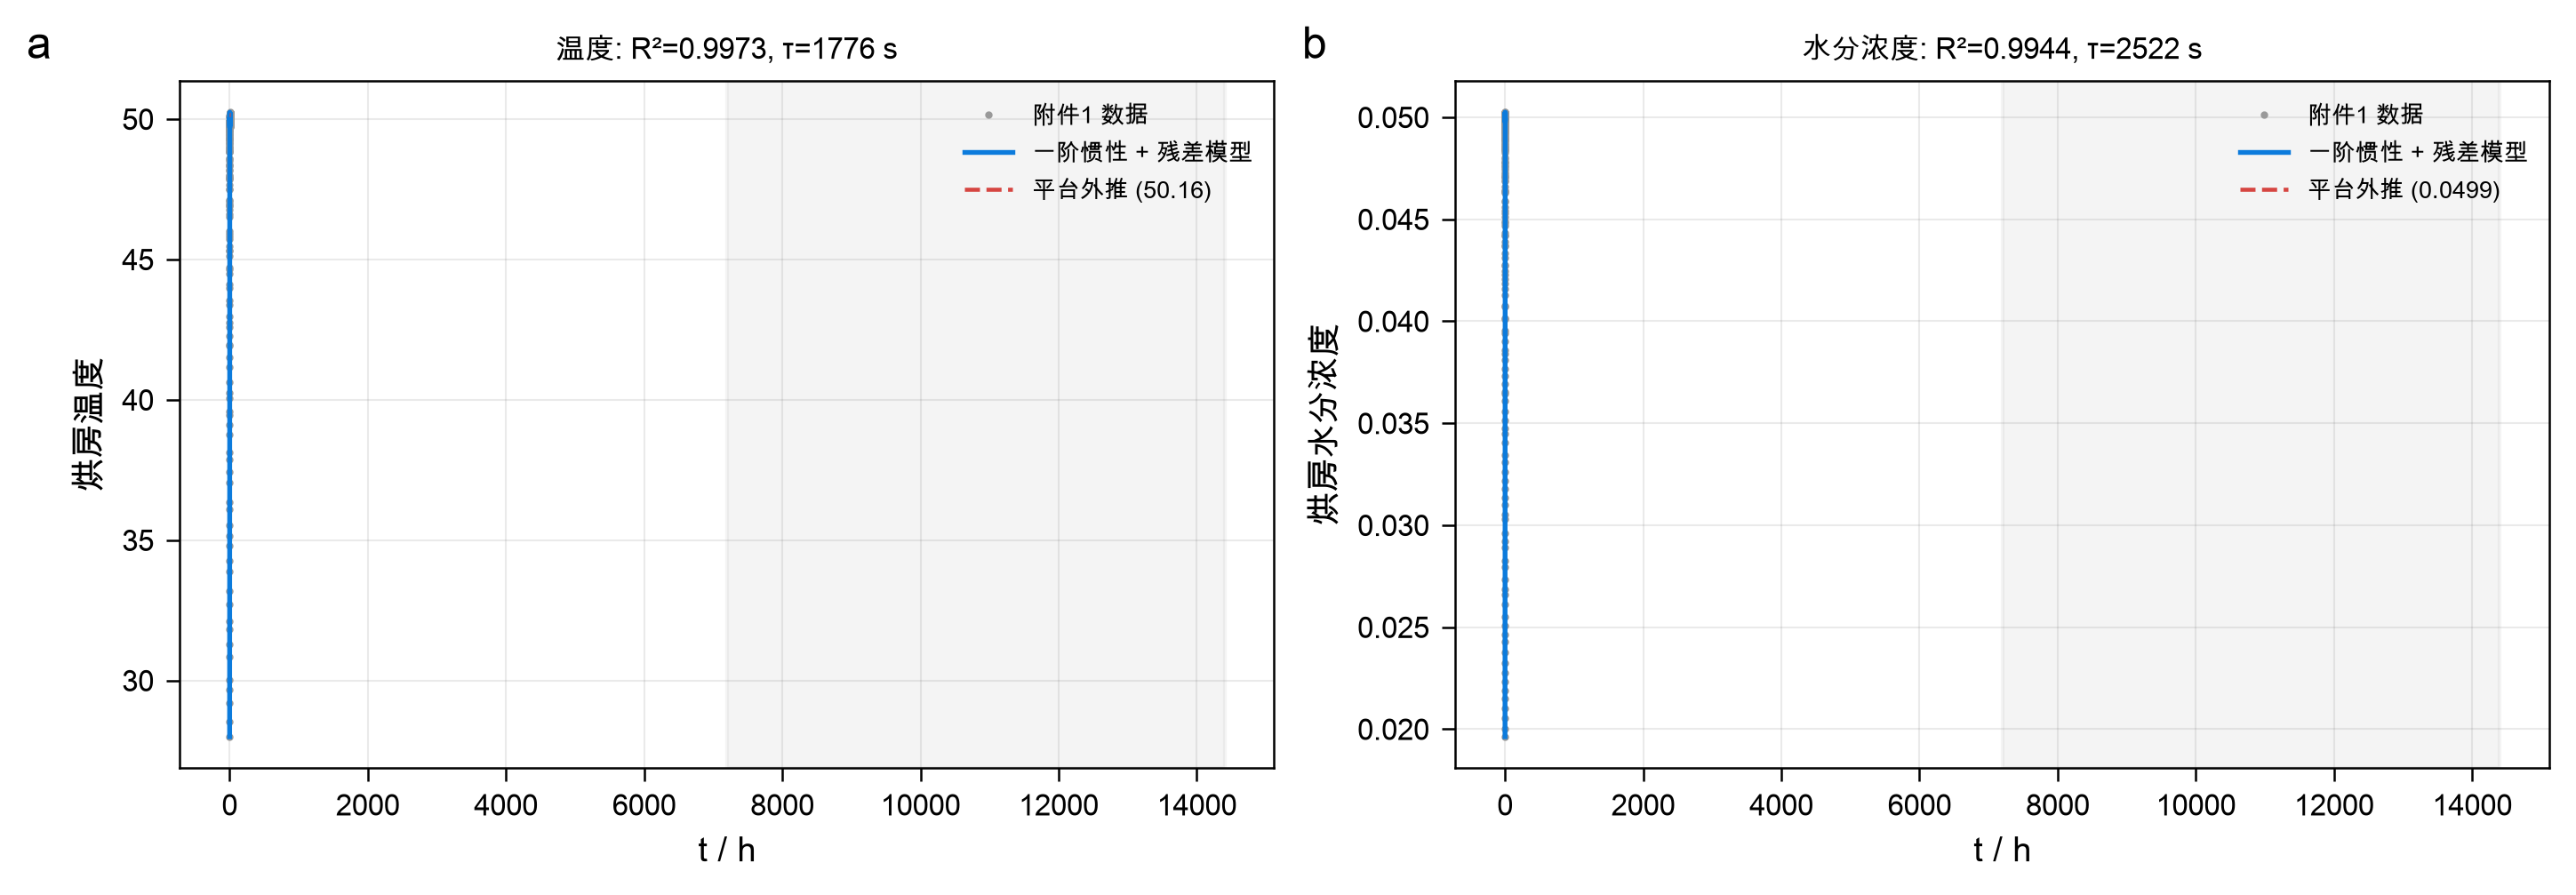
\includegraphics[width=0.95\textwidth]{fig6_env_model.png}
\caption{烘房环境的一阶惯性辨识。数据点、辨识模型与平台期统计区间（阴影）。
左：温度（$R^2=0.9973$，$\tau=1776$ s）；右：水分浓度（$R^2=0.9944$，
$\tau=2522$ s）。}
\label{fig:env}
\end{figure}

\subsubsection{温度场解析解}

预热阶段温度场满足常物性轴对称热传导方程

\begin{equation}
\rho c_p\frac{\partial T}{\partial t}=\frac{k}{r}\frac{\partial}{\partial r}\left(r\frac{\partial T}{\partial r}\right)
\end{equation}
\begin{equation}
T(r,0)=T_0,\qquad \left.\frac{\partial T}{\partial r}\right|_{r=0}=0,\qquad
-\left.k\frac{\partial T}{\partial r}\right|_{r=R}=h\big(T(R,t)-T_{env}(t)\big)
\end{equation}

（$\rho=820$ kg/m$^3$、$c_p=2600$ J/(kg·K)、$k=0.36$ W/(m·K)、
$h=25$ W/(m$^2$·K)，附录 2）。对流边界的特征值问题为
$\lambda J_1(\lambda)=\mathrm{Bi}\,J_0(\lambda)$，$\mathrm{Bi}=hR/k=1.39$。
对该特征展开应用 Duhamel 原理（推导过程见附录 A），指数边界主项可显式求积，
残差经递归卷积修正，最终

\begin{equation}
T(r,t)=T_{fit}(t)-\Delta T\sum_{n=1}^{80}A_n J_0\!\left(\frac{\lambda_n r}{R}\right)g_n(t)
+\delta(t)-\sum_{n=1}^{80}A_n J_0\!\left(\frac{\lambda_n r}{R}\right)I_n(t)
\end{equation}

其中 $T_{fit}(t)=T_\infty-\Delta T\,e^{-t/\tau}$ 为辨识主项，$\delta(t)$ 为
环境残差，$g_n$、$I_n$ 与系数 $A_n$ 的定义见附录 A。该式对任意输出时刻
无需时间步进，级数截断误差在 $10^{-9}$ 量级，满足 4 位小数要求；$\tau\to0$
时退化为阶跃边界响应，与 Bessel 级数解逐点一致到 $5\times10^{-9}$。
这一解析解同时作为谱配点求解器的独立基准（图~\ref{fig:duhamel}）。

\begin{figure}[H]
\centering
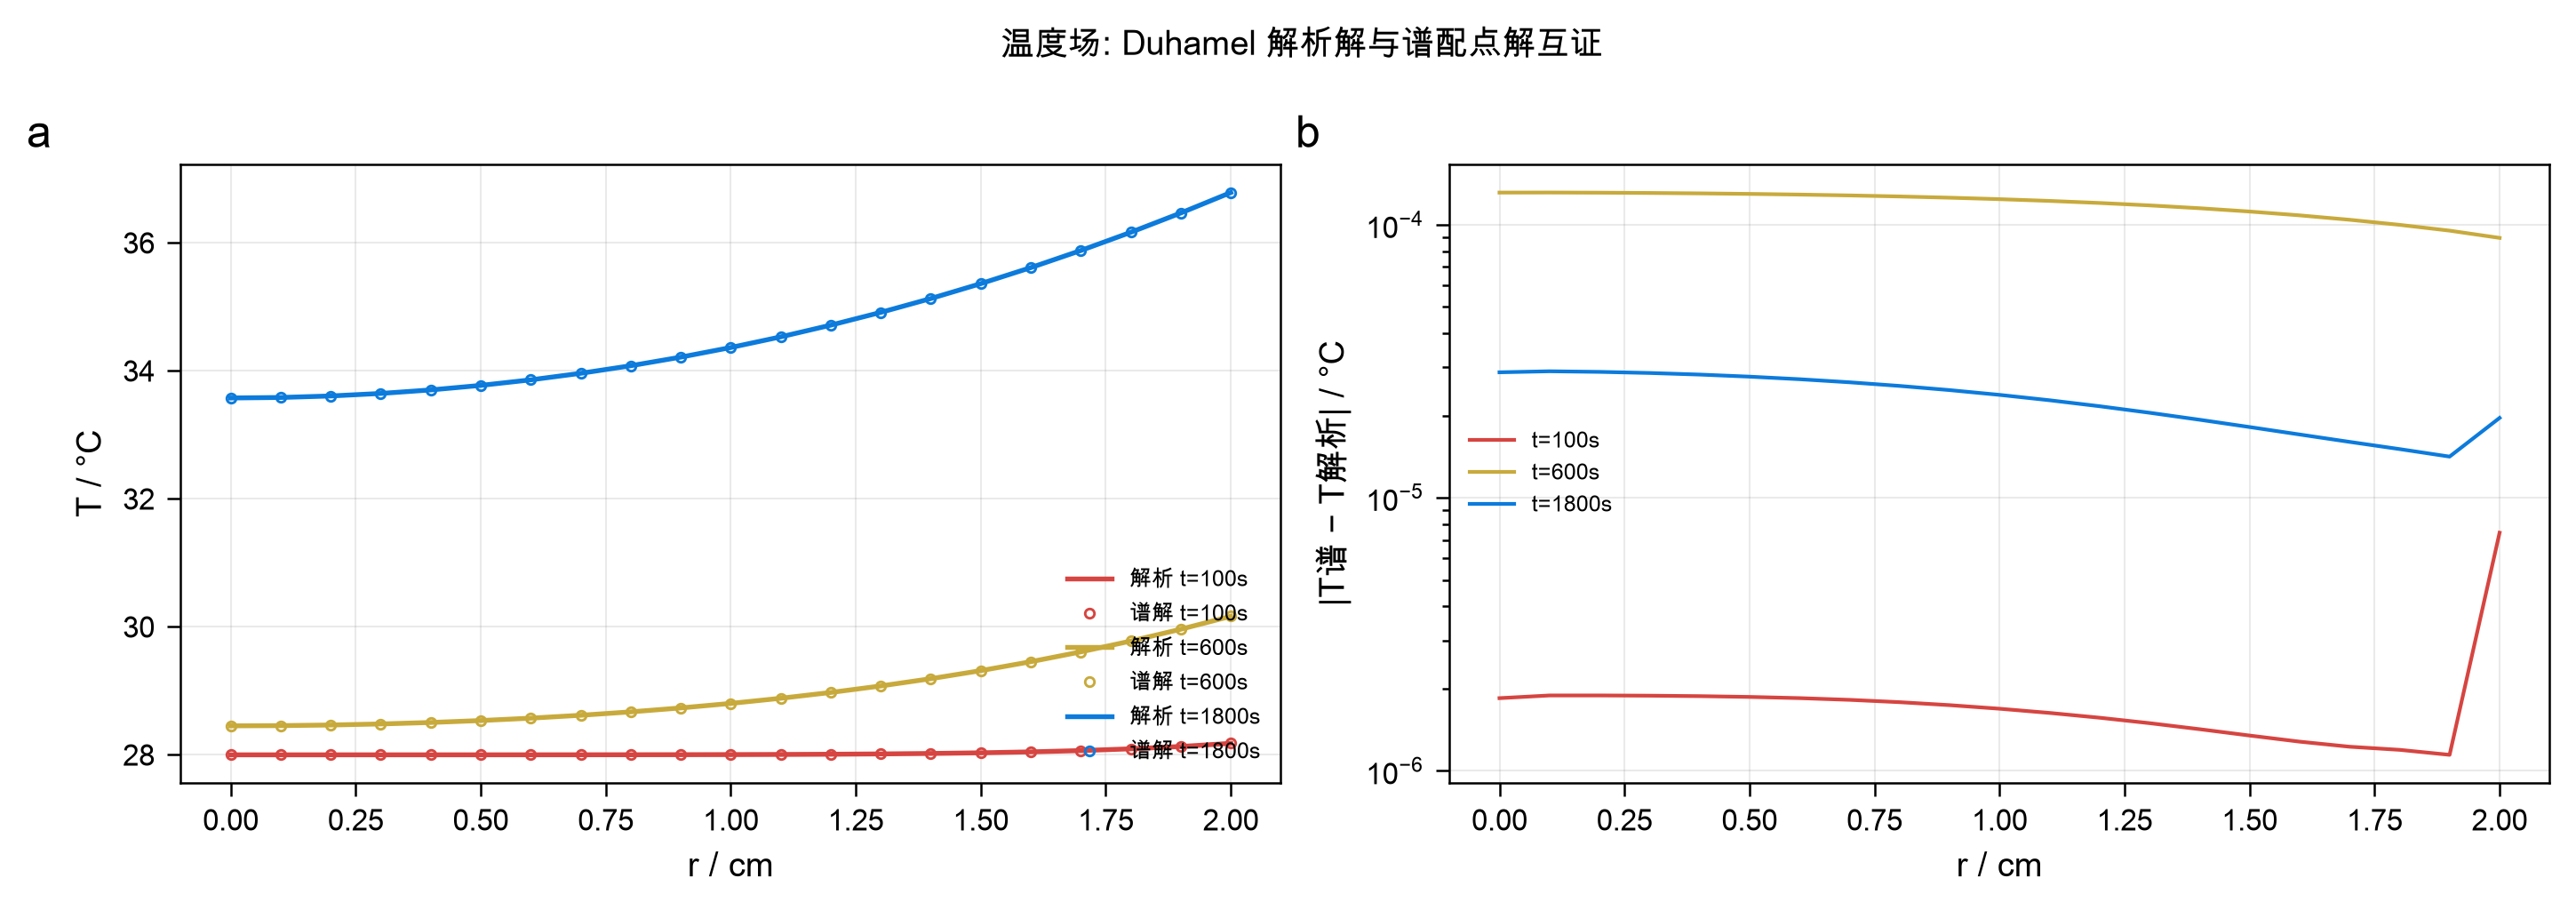
\includegraphics[width=0.95\textwidth]{fig2_duhamel.png}
\caption{温度场解析解与谱配点解的对比（a）及逐点偏差（b）。最大偏差
$1.6\times10^{-4}$\,°C，两种求解方式相互印证。}
\label{fig:duhamel}
\end{figure}

\subsubsection{水分场与统一数值离散}

水分场满足非线性扩散方程

\begin{equation}
\frac{\partial C}{\partial t}=\frac{1}{r}\frac{\partial}{\partial r}\left(r\,D(C)\frac{\partial C}{\partial r}\right),\qquad
D(C)=7\times10^{-9}e^{-0.89/C}
\end{equation}

初值 $C(r,0)=2.55$，表面条件 $-D\,\partial C/\partial r=\beta(C-C_{env})$，
$\beta=8\times10^{-7}$ m/s。温度方程与水分方程没有直接的双向作用（热物性
为常数，$D$ 不含温度），水分方程经 $D(C)$ 单向依赖于自身场。

空间离散采用 Chebyshev--Gauss--Lobatto 谱配点（$N$ 个模式，$r=R(1-x)/2$
映射），一阶微分矩阵按 Trefethen 公式给出\cite{trefethen}；扩散项按乘积
链式离散，即对 $rD(C)\,C_r$ 整体微分，该形式在轴心处保持正则（展开形式
$C_{rr}+C_r/r$ 在轴心附近的谱离散不稳定，具体分析见附录 B）。轴心与表面
两个边界节点不作为时间积分状态，而在每次右端求值中由对称条件与 Robin
条件解出（边界方程求解与选支处理的细节见附录 B）。半离散系统用自适应
隐式 BDF 积分，末位 Chebyshev 系数作为后验误差指示\cite{gasparin}：
问题一解在 $t=1800$ s 时末位系数 $5.1\times10^{-13}$（图~\ref{fig:spectral}），
远低于 4 位小数阈值。该离散框架为问题二至四的统一求解内核。

\begin{figure}[H]
\centering
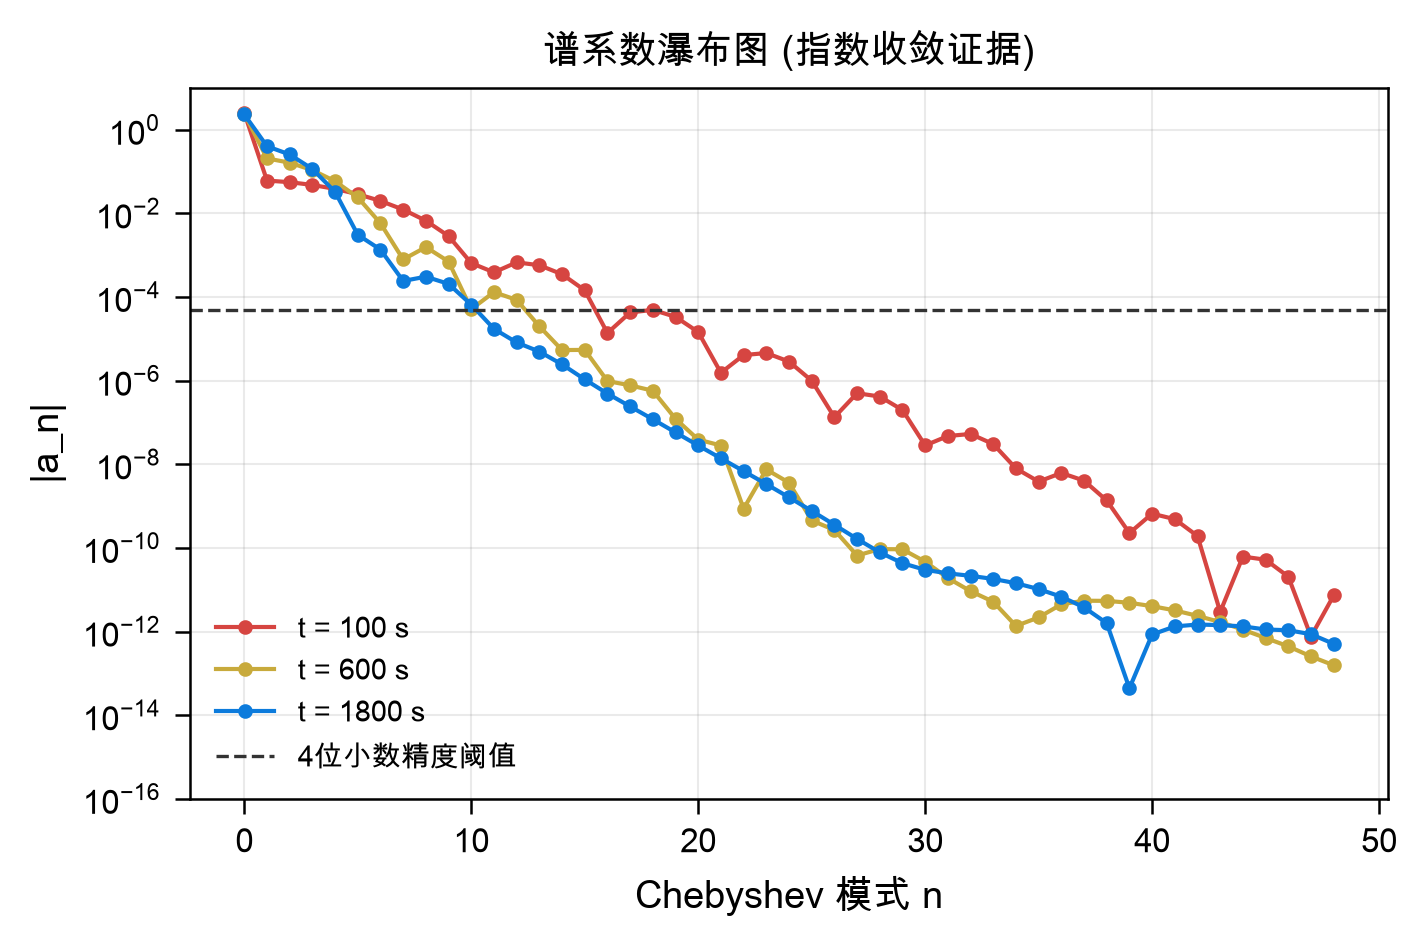
\includegraphics[width=0.62\textwidth]{fig1_spectral.png}
\caption{谱系数随模式数指数衰减（$t=1800$ s）。末位系数 $5\times10^{-13}$
远低于 4 位小数精度阈值 $5\times10^{-5}$。}
\label{fig:spectral}
\end{figure}

\subsubsection{结果}

表~\ref{tab:q1t}、\ref{tab:q1c}（分别按题目表 1、表 2 格式输出，完整数据
见 result1.xlsx）：30 min 内表面温度由 28.00\,°C 升至 36.79\,°C
（100 s 时 28.18\,°C），中心升至 33.58\,°C；表面含水率由 2.5500 降至
1.5102 kg/kg，中心保持 2.5500 kg/kg。图~\ref{fig:preheat} 以二维热图
与径向剖面给出时空演化：温度场整体爬升并形成径向梯度，水分仅在表面薄层
下降。这与无量纲估计一致（$\mathrm{Fo}_T=0.76$、$\mathrm{Fo}_m=0.022$）：
预热阶段工艺目标是快速均温、尽量保持内部水分。

\begin{figure}[H]
\centering
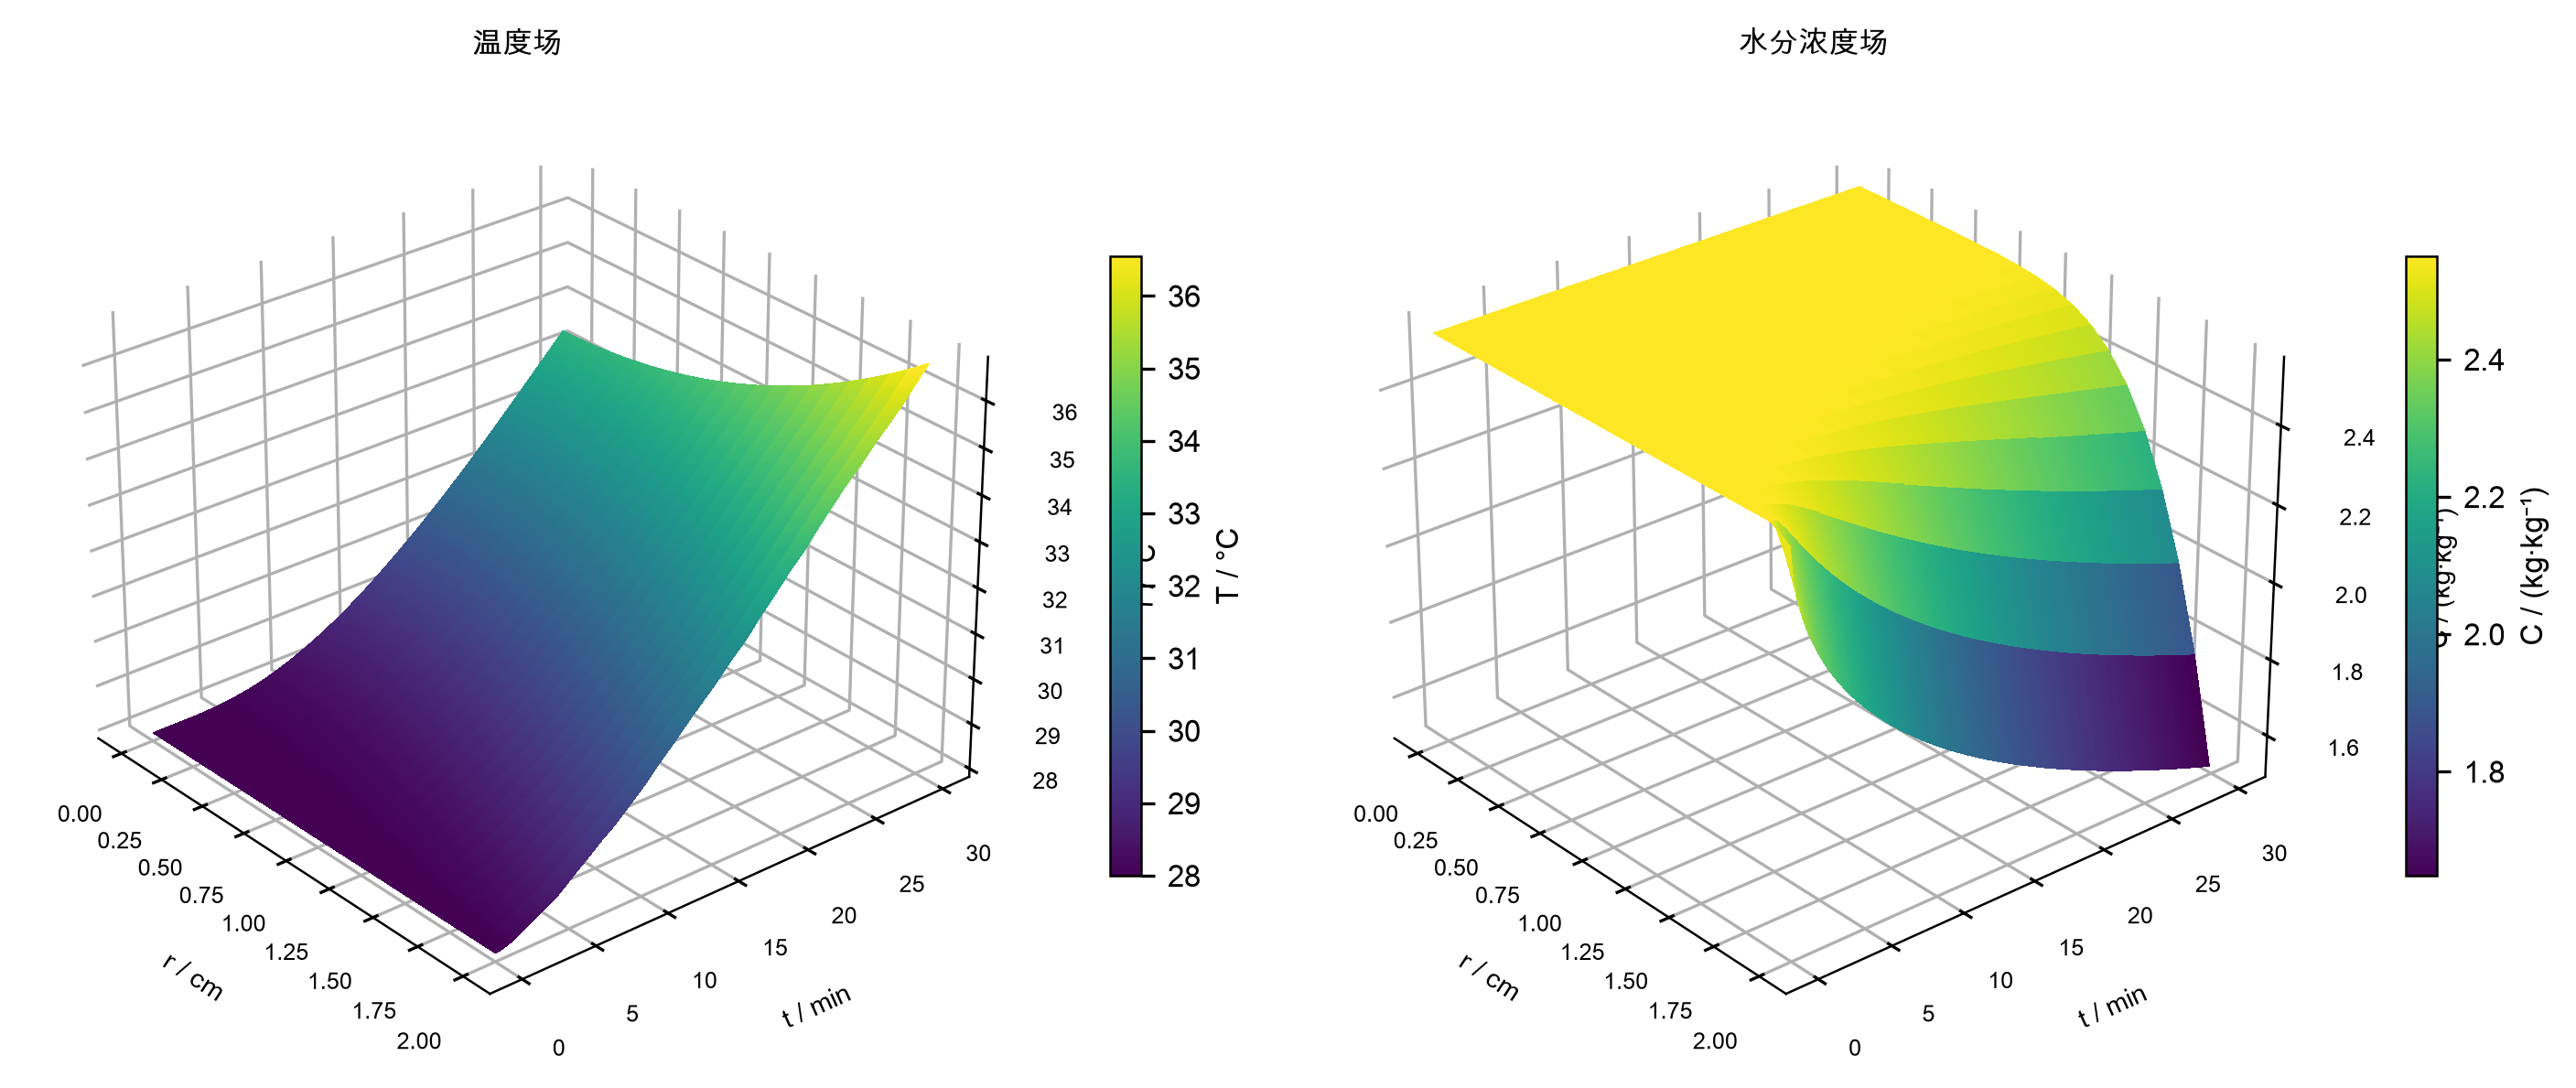
\includegraphics[width=0.95\textwidth]{fig3_preheat.png}
\caption{预热阶段时空演化（二维热图，上）与典型时刻径向剖面（下）。
左列温度，右列水分浓度。}
\label{fig:preheat}
\end{figure}

\begin{table}[H]
\centering
\caption{30 分钟内药材的温度（按题目表 1 的格式要求输出，完整数据见 result1.xlsx）}
\label{tab:q1t}
\begin{tabular}{c|ccccc}
\toprule
时间/s & 0 cm & 0.5 cm & 1 cm & 1.5 cm & 2 cm \\
\midrule
100 & 28.0000 & 28.0003 & 28.0038 & 28.0317 & 28.1792 \\
300 & 28.0405 & 28.0632 & 28.1509 & 28.3668 & 28.8483 \\
600 & 28.4530 & 28.5357 & 28.8035 & 29.3156 & 30.1646 \\
900 & 29.3240 & 29.4581 & 29.8756 & 30.6164 & 31.7295 \\
1200 & 30.5428 & 30.7099 & 31.2225 & 32.1128 & 33.4284 \\
1500 & 31.9960 & 32.1871 & 32.7665 & 33.7471 & 35.1196 \\
1800 & 33.5758 & 33.7723 & 34.3644 & 35.3624 & 36.7859 \\
\bottomrule
\end{tabular}
\end{table}

\begin{table}[H]
\centering
\caption{30 分钟内药材的水分浓度（按题目表 2 的格式要求输出，单位 kg/kg）}
\label{tab:q1c}
\begin{tabular}{c|ccccc}
\toprule
时间/s & 0 cm & 0.5 cm & 1 cm & 1.5 cm & 2 cm \\
\midrule
100 & 2.5500 & 2.5500 & 2.5500 & 2.5500 & 2.2470 \\
300 & 2.5500 & 2.5500 & 2.5500 & 2.5492 & 2.0508 \\
600 & 2.5500 & 2.5500 & 2.5500 & 2.5353 & 1.8770 \\
900 & 2.5500 & 2.5500 & 2.5497 & 2.5045 & 1.7547 \\
1200 & 2.5500 & 2.5500 & 2.5482 & 2.4646 & 1.6586 \\
1500 & 2.5500 & 2.5499 & 2.5445 & 2.4206 & 1.5787 \\
1800 & 2.5500 & 2.5497 & 2.5383 & 2.3755 & 1.5102 \\
\bottomrule
\end{tabular}
\end{table}


\subsubsection{验证}

\begin{enumerate}
\item 解析基准：谱配点温度解与 5.1.2 解析解逐点对比，最大偏差
$1.6\times10^{-4}$\,°C（图~\ref{fig:duhamel}）；
\item 常扩散系数情形的谱解与 Bessel 级数解偏差 $9.5\times10^{-9}$；
\item 独立算法交叉验证：与有限体积法求解器（400 节点，网格收敛验证后）
对比，表~\ref{tab:q1t}、\ref{tab:q1c} 逐项 4 位小数一致。
\end{enumerate}

% ============ §5.2 问题二 ============
\subsection{问题二：变物性双向热湿耦合模型}

\subsubsection{变物性与双向耦合}

整个烘干过程（预热平衡 + 恒温干燥）采用附录 3 的经验公式：$\rho,c_p,k$
依赖含水率 $C$，扩散系数 $D$ 同时依赖 $C$ 与温度 $T$：

\begin{equation}
\rho=650+128C,\qquad c_p=1450+2736\frac{C}{C+1},\qquad k=0.21+0.38\frac{C}{C+1}
\end{equation}
\begin{equation}
D=2.4\times10^{-3}e^{-0.45/C}e^{-3850/T_K}
\end{equation}

（$T_K$ 取开尔文）。耦合在整个求解域内双向进行：含水率 $C$ 通过
$\rho,c_p,k$ 改变热惯性与导热能力；温度 $T$ 通过 Arrhenius 项
$e^{-3850/T_K}$ 改变水分迁移速率。控制方程为

\begin{equation}
\rho(C)c_p(C)\frac{\partial T}{\partial t}=\frac{1}{r}\frac{\partial}{\partial r}\left(r k(C)\frac{\partial T}{\partial r}\right),\qquad
\frac{\partial C}{\partial t}=\frac{1}{r}\frac{\partial}{\partial r}\left(r D(C,T)\frac{\partial C}{\partial r}\right)
\end{equation}

边界条件与问题一相同（$h=25$ W/(m$^2$·K)、$\beta=8\times10^{-7}$ m/s），
环境条件两段拼接：0--4 h 用 5.1.1 的辨识模型，$t>4$ h 用平台外推值。

其中扩散系数的变化范围决定了问题的数值性质：$D$ 在 $C=2.55$、
$T=50$\,°C 时约 $1.3\times10^{-8}$ m$^2$/s，含水率降至 0.05 时约
$10^{-12}$ m$^2$/s——下降约 \textbf{4 个数量级}。干燥由此进入减速段：表面在约
12 h 即接近环境平衡值，而中心含水率的下降持续近 3 天。

\subsubsection{耦合求解与空间收敛}

数值求解沿用 5.1.3 的统一离散：两个场的内部节点拼接为
$\mathbf{y}=[\mathbf{T};\mathbf{C}]$（$2(N-1)$ 维），轴心与表面边界条件在
每次右端求值中由对称条件与 Robin 条件联立解出，时间积分用自适应隐式 BDF
（相对容差 $10^{-8}$，积分 72 h）。

空间分辨率是本问的关键数值问题。$N=48$ 时末位谱系数 $1.3\times10^{-3}$，
72 h 中心含水率 $0.1515$，与独立有限体积法参考解（$0.1380$）偏差
$0.0135$——干燥锋面未被充分分辨。加密后：

\begin{table}[H]
\centering
\caption{谱模式数收敛（72 h 中心含水率）}
\label{tab:conv}
\begin{tabular}{cccc}
\toprule
$N$ & 48 & 96 & 128 \\
\midrule
中心含水率 @72h & 0.1515 & 0.1386 & 0.1379 \\
末位谱系数 & $1.3\times10^{-3}$ & $6.8\times10^{-5}$ & $1.2\times10^{-5}$ \\
\bottomrule
\end{tabular}
\end{table}

$N=96$ 起与有限体积法一致到 \textbf{$6\times10^{-4}$}，$N=128$ 进一步收敛
（图~\ref{fig:conv}）。本文全部提交结果取 $N=128$；问题一剖面光滑，
$N=48$ 已足够（末位系数 $5\times10^{-13}$）。

\begin{figure}[H]
\centering
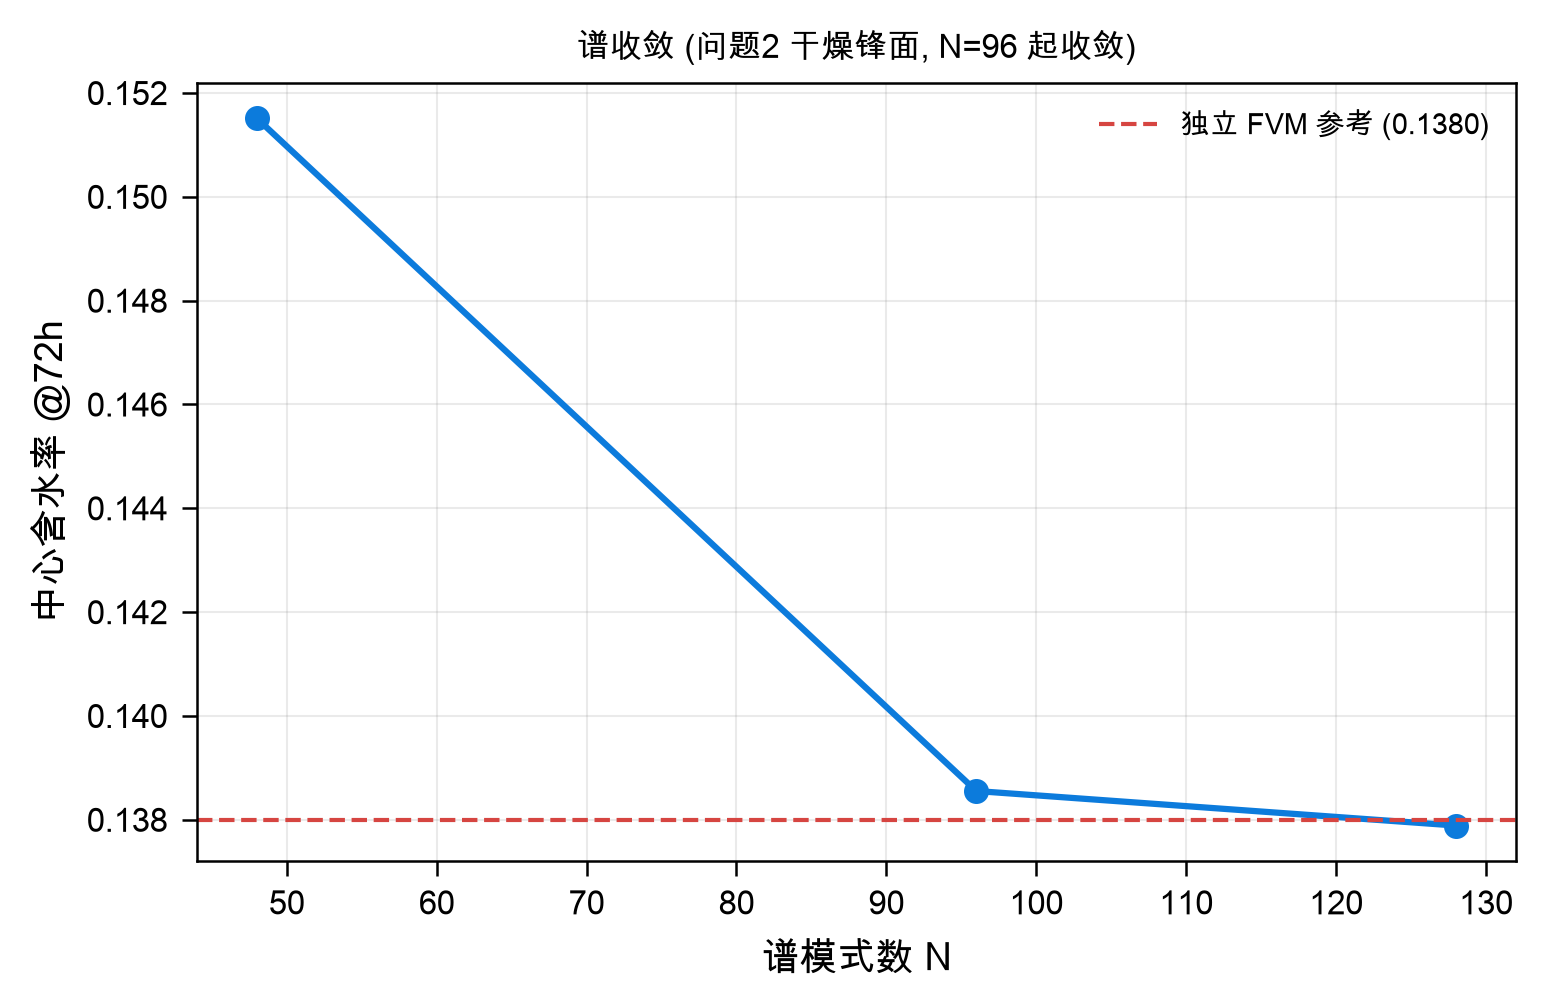
\includegraphics[width=0.62\textwidth]{fig11_convergence.png}
\caption{空间收敛：72 h 中心含水率随谱模式数的变化。$N=48$ 欠分辨，
$N=96$ 起与独立有限体积法参考解（虚线）一致。}
\label{fig:conv}
\end{figure}

\subsubsection{结果与讨论}

表~\ref{tab:q2t}、\ref{tab:q2c}（分别按题目表 3、表 4 格式输出，完整数据
见 result2.xlsx）：3 h 时温度场已均匀（表面 49.97\,°C、中心 49.85\,°C），
表面含水率降至 1.008 kg/kg、中心 1.766 kg/kg。图~\ref{fig:gamma} 给出
时间尺度比 $\Gamma=\alpha/D$ 的时空分布：湿态约 10，干态升至 $10^5$。
$\Gamma$ 小时热、湿两场的时间尺度接近；$\Gamma$ 大时温度场相对水分场
快速趋于准稳态，总干燥过程逐渐受水分扩散控制。这与 6.2 节中烘干时长对
换热系数不敏感的结果一致。

\begin{table}[H]
\centering
\caption{3 小时内药材的温度（按题目表 3 的格式要求输出，单位 °C）}
\label{tab:q2t}
\begin{tabular}{c|ccccc}
\toprule
时间/h & 0 cm & 0.5 cm & 1 cm & 1.5 cm & 2 cm \\
\midrule
0.5 & 32.1896 & 32.3824 & 32.9661 & 33.9610 & 35.4133 \\
1.0 & 40.3821 & 40.5541 & 41.0610 & 41.8784 & 42.9990 \\
1.5 & 45.8471 & 45.9352 & 46.1932 & 46.6055 & 47.1395 \\
2.0 & 48.4504 & 48.4882 & 48.5985 & 48.7736 & 49.0032 \\
2.5 & 49.4670 & 49.4793 & 49.5137 & 49.5646 & 49.6618 \\
3.0 & 49.8494 & 49.8553 & 49.8746 & 49.9101 & 49.9667 \\
\bottomrule
\end{tabular}
\end{table}

\begin{table}[H]
\centering
\caption{3 小时内药材的水分浓度（按题目表 4 的格式要求输出，单位 kg/kg）}
\label{tab:q2c}
\begin{tabular}{c|ccccc}
\toprule
时间/h & 0 cm & 0.5 cm & 1 cm & 1.5 cm & 2 cm \\
\midrule
0.5 & 2.5499 & 2.5489 & 2.5256 & 2.3257 & 1.6486 \\
1.0 & 2.5257 & 2.4948 & 2.3578 & 2.0230 & 1.4711 \\
1.5 & 2.3861 & 2.3256 & 2.1344 & 1.8020 & 1.3476 \\
2.0 & 2.1708 & 2.1084 & 1.9236 & 1.6259 & 1.2311 \\
2.5 & 1.9566 & 1.9006 & 1.7360 & 1.4720 & 1.1166 \\
3.0 & 1.7662 & 1.7165 & 1.5702 & 1.3333 & 1.0081 \\
\bottomrule
\end{tabular}
\end{table}


\begin{figure}[H]
\centering
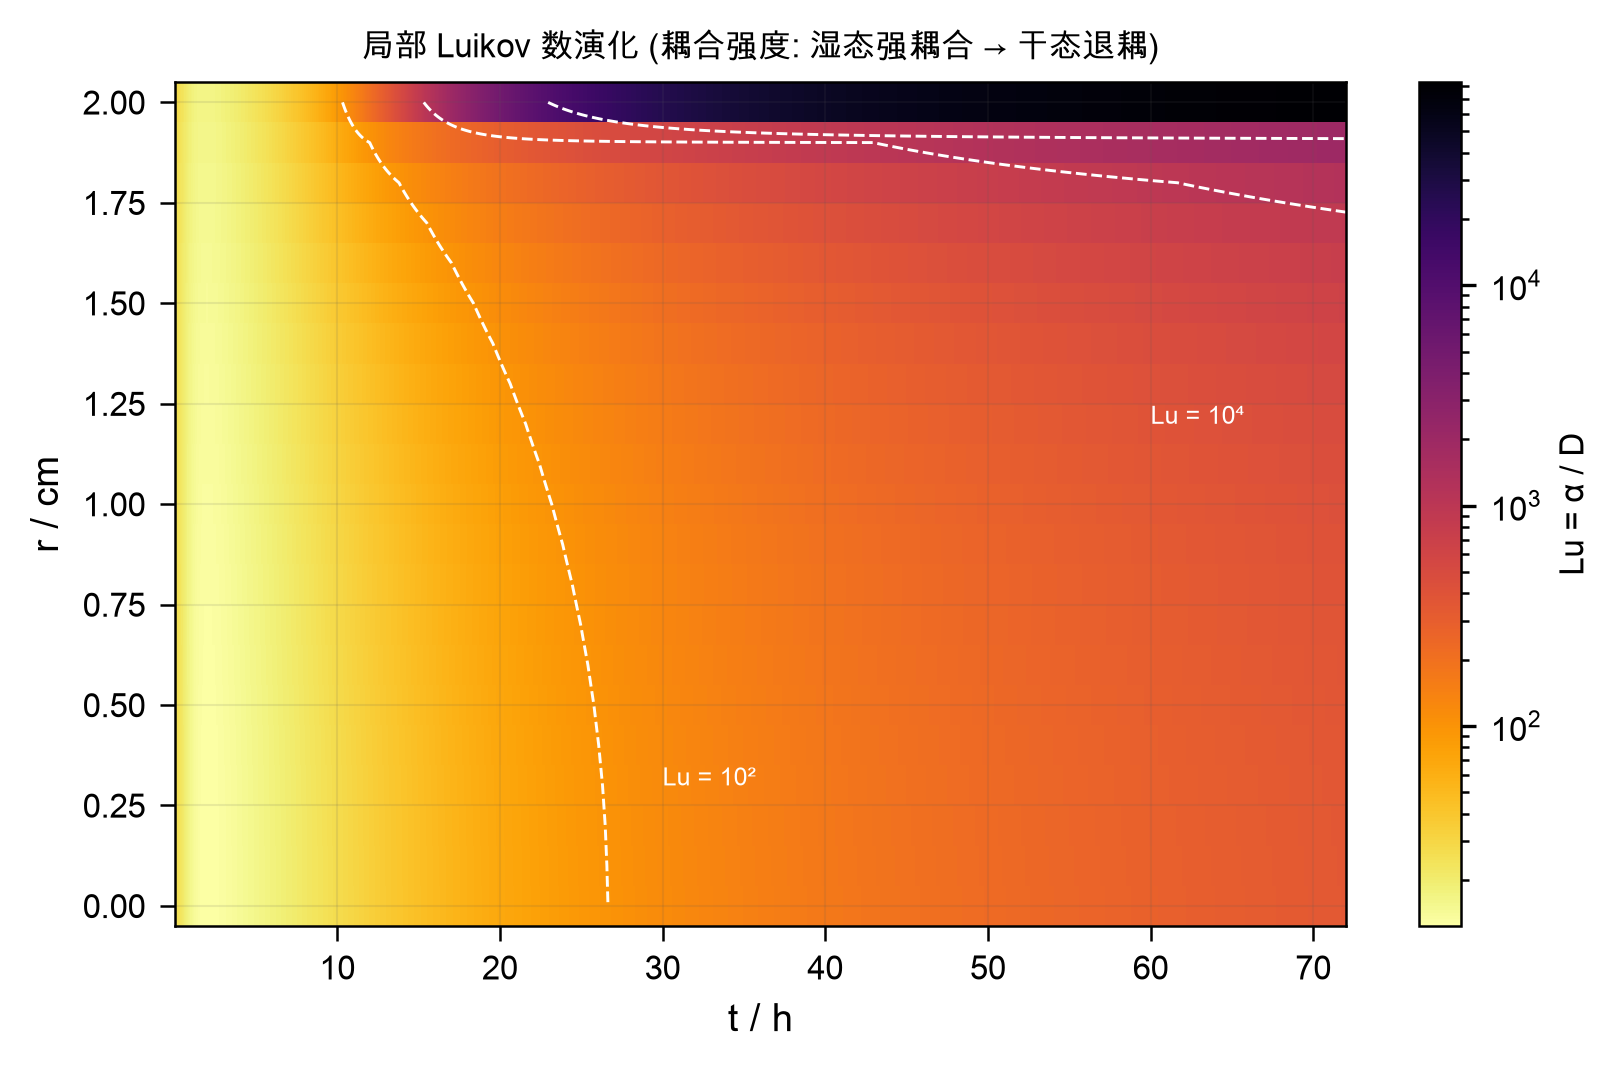
\includegraphics[width=0.62\textwidth]{fig5_lu.png}
\caption{时间尺度比 $\Gamma=\alpha/D$ 的时空分布（对数色标）。$\Gamma$ 增大
表示热扩散相对水分扩散更快，温度场更快趋于准稳态。}
\label{fig:gamma}
\end{figure}

% ============ §5.3 问题三 ============
\subsection{问题三：烘干时长判定}

烘干要求药材各处水分浓度低于 0.15 kg/kg。定义
\begin{equation}
C_{\max}(t)=\max_{0\le r\le R}C(r,t)
\end{equation}
程序在问题二的解上以 60 s 分辨率对 $C_{\max}(t)$ 做实际扫描（输出网格
21 个径向点取最大值），寻找首个满足 $C_{\max}(t)<0.15$ 的时刻：

\begin{equation}
t_{end}=208200\ \mathrm{s}=\mathbf{57.83\ h}
\end{equation}

数值解在全部输出时刻均保持由中心向表面单调下降（逐时刻检查通过），
$C_{\max}$ 始终出现在 $r=0$ 处，因此后续分析与图表等价地监测
$C(0,t)$。跨越细节：$t=208140$ s 时中心含水率 $0.150002$，$t=208200$ s 时
$0.149983$（图~\ref{fig:criterion}）。需要注意，跨越处中心曲线衰减速率仅
约 $10^{-3}$ /h，判据对数值精度敏感：本文谱配点（$N=128$）给出 57.83 h，
独立有限体积法（400 节点、800 节点验证）给出 57.77 h，两种独立离散
相差 \textbf{0.06 h}。这一敏感性在表~\ref{tab:q3} 的最后一行体现为恰好跨过判据
的数值。

\begin{figure}[H]
\centering

\includegraphics[width=0.95\textwidth]{fig8_criterion.png}
\caption{中心/表面含水率轨迹与 0.15 判据线（内嵌 56.5--60.5 h 放大图）。}
\label{fig:criterion}
\end{figure}

\begin{figure}[H]
\centering

\includegraphics[width=0.95\textwidth]{fig4_front.png}
\caption{全流程水分浓度二维热图（左）与干燥锋面位置随时间的变化
（右，虚线为 $\sqrt{t}$ 参考）。}
\label{fig:front}
\end{figure}

与附件 2 的半径收缩平台（约 70 h）比较，57.83 h 与之处于同一物理量级
（收缩阶段含水率已很低，两种现象的时间尺度自洽），不构成对烘干时长的
独立定量验证。

\begin{table}[H]
\centering
\caption{药材烘干过程的水分浓度（按题目表 5 的格式要求输出，单位 kg/kg；末行为判据跨越时刻）}
\label{tab:q3}
\begin{tabular}{c|ccccc}
\toprule
时间/h & 0 cm & 0.5 cm & 1 cm & 1.5 cm & 2 cm \\
\midrule
6 & 1.0172 & 0.9884 & 0.9017 & 0.7550 & 0.5326 \\
12 & 0.4564 & 0.4434 & 0.4032 & 0.3298 & 0.1640 \\
18 & 0.2990 & 0.2917 & 0.2688 & 0.2254 & 0.0844 \\
24 & 0.2380 & 0.2329 & 0.2168 & 0.1856 & 0.0663 \\
30 & 0.2063 & 0.2020 & 0.1892 & 0.1642 & 0.0597 \\
36 & 0.1865 & 0.1827 & 0.1718 & 0.1505 & 0.0565 \\
42 & 0.1727 & 0.1693 & 0.1597 & 0.1408 & 0.0547 \\
48 & 0.1623 & 0.1593 & 0.1507 & 0.1335 & 0.0536 \\
54 & 0.1543 & 0.1516 & 0.1437 & 0.1278 & 0.0529 \\
57.83 & 0.1500 & 0.1474 & 0.1399 & 0.1247 & 0.0525 \\
\bottomrule
\end{tabular}
\end{table}


% ============ §5.4 问题四 ============
\subsection{问题四：随体坐标下干基含水率守恒方程}

\subsubsection{干基含水率的物质守恒}

问题四中半径随失水收缩，$R(t)$ 由附件 2 给定（2.00$\to$1.198 cm，保形
三次样条插值，$t>252000$ s 平台外推）。收缩使求解域随时间变化，直接在内
部固定网格上离散需要处理移动边界两侧的守恒关系。本文改用随体坐标
（网格随材料一起运动），利用干基含水率的定义简化方程。

干基含水率 $C=m_w/m_s$ 依附于干物质：固定一组随体坐标，就固定了一团
干物质，其质量 $m_s$ 不随时间变化。设材料速度 $u=\dot R\,r/R$（径向
仿射收缩），干物质密度 $\rho_s\propto1/R^2$ 均匀压实，水分守恒的欧拉
形式为

\begin{equation}
\frac{\partial(\rho_s C)}{\partial t}+\nabla\cdot(u\,\rho_s C)=\nabla\cdot(\rho_s D\nabla C)
\end{equation}

将 $\rho_s$ 与 $u$ 的表达式代入并变换到随体坐标，对流项、体积膨胀项与
密度变化项相互消去（推导见附录 A），得到

\begin{equation}
\left.\frac{\partial C}{\partial t}\right|_{g}=\frac{1}{r}\frac{\partial}{\partial r}\left(rD(C,T)\frac{\partial C}{\partial r}\right)
\end{equation}

即：在随体坐标下，干基含水率的演化仅由相对扩散决定。一个直接的检验是
均匀场情形：$C$ 为常数时方程右端恒为零，含水率保持不变——收缩本身不会
产生虚假的含水率变化。这也说明径向仿射收缩是本文的\textbf{关键假设}：题目只提供
$R(t)$ 的径向数据，各向异性或轴向收缩未建模。

物性换为附录 4（$\rho=760+90C$、$c_p=1850+2150C/(C+1)$、
$k=0.12+0.20C/(C+1)$、$D=4.2\times10^{-4}e^{-0.30/C}e^{-3850/T_K}$），
温度方程同构。数值实现：随体网格的微分矩阵按 $R(t)$ 逐次更新，边界条件
求解与 5.2.2 相同，$N=96$、相对容差 $10^{-8}$。

\subsubsection{结果与控制变量分解}

问题四的设置相对问题三同时改变了两件事：物性体系（附录 3 $\to$ 附录 4）与
求解域（固定半径 $\to$ 收缩）。二者对烘干时长的影响方向相反，直接比较
两个问题的时间差无法将全部差异归因于收缩。为此增设一个控制变量基准：

\begin{table}[H]
\centering
\caption{问题四的对照设置与烘干时长（判据 $C_{\max}<0.15$）}
\label{tab:control}
\begin{tabular}{lccc}
\toprule
设置 & 物性 & 半径 & 烘干时长 \\
\midrule
问题三 & 附录 3 & $R=2$ cm 固定 & 57.83 h \\
基准 A（本文增设） & 附录 4 & $R=2$ cm 固定 & $>150$ h（模拟至 150 h 仍未达标） \\
模型 B（问题四） & 附录 4 & 附件 2 $R(t)$ & 51.15 h \\
\bottomrule
\end{tabular}
\end{table}

据此把问题三到问题四的总差异分解为两部分：
\begin{equation}
\Delta t_{total}=57.83-51.15=6.68\ \mathrm{h}
=\underbrace{\Delta t_{props}}_{\text{物性体系}}+\underbrace{\Delta t_{shrink}}_{\text{纯几何收缩}}
\end{equation}
其中 $\Delta t_{props}=t_{Q3}-t_{A}<0$（附录 4 的扩散系数在湿态约为附录 3
的五分之一，物性变化使干燥变慢，幅度超过 92 h），
$\Delta t_{shrink}=t_{A}-t_{B}>98.85$ h（收缩使扩散路径缩短，加速幅度
超过 98 h，即相对基准 A 缩短约三分之二）。两重效应相互抵消后净得 6.68 h。
**若仅比较问题三与问题四的总差异，会严重低估收缩的加速作用。**

\begin{figure}[H]
\centering

\includegraphics[width=0.95\textwidth]{fig9_shrink.png}
\caption{（a）附件 2 实测半径与插值轨迹；（b）三种设置的中心含水率对比
（问题三 / 附录 4 固定半径 / 附录 4 收缩）；（c）收缩--失水关系。}
\label{fig:shrink}
\end{figure}

\begin{table}[H]
\centering
\caption{药材烘干过程的水分浓度（表 6, 收缩模型, kg/kg; 末列为药材表面处的值, 最后一列为该时刻的半径）}
\begin{tabular}{c|ccccc}
\toprule
时间/h & 0 cm & 0.5 cm & 1.0 cm & 药材表面 & $R(t)$/cm \\
\midrule
6 & 1.7192 & 1.5374 & 1.0223 & 0.4202 & 1.374 \\
12 & 0.7379 & 0.6548 & 0.4084 & 0.1668 & 1.248 \\
18 & 0.4090 & 0.3689 & 0.2398 & 0.0891 & 1.214 \\
24 & 0.2853 & 0.2612 & 0.1791 & 0.0672 & 1.204 \\
30 & 0.2265 & 0.2095 & 0.1493 & 0.0594 & 1.201 \\
36 & 0.1929 & 0.1798 & 0.1317 & 0.0558 & 1.200 \\
42 & 0.1713 & 0.1605 & 0.1200 & 0.0540 & 1.200 \\
48 & 0.1562 & 0.1469 & 0.1116 & 0.0529 & 1.200 \\
51.15 & 0.1500 & 0.1412 & 0.1080 & 0.0525 & 1.200 \\
\bottomrule
\end{tabular}
\end{table}


% ============ §6 数值验证与灵敏度 ============
\section{数值验证与灵敏度分析}

\subsection{多层次数值验证}

本文对数值结果做了三类验证，其结论已在各节给出，此处汇总。

\textbf{（1）解析与制造解验证。} 温度场：谱配点解与 5.1.2 解析解偏差
$1.6\times10^{-4}$\,°C；常扩散系数情形与 Bessel 级数解偏差
$9.5\times10^{-9}$。水分场（非线性）：构造光滑制造解并反推解析强迫项
\cite{roache}，谱解与制造解偏差 $6.1\times10^{-9}$；时间容差从 $10^{-8}$
收紧到 $10^{-12}$ 时误差由 $2.7\times10^{-7}$ 降至 $2.1\times10^{-10}$
（图~\ref{fig:mms}），表明误差受容差控制而非格式缺陷。

\begin{figure}[H]
\centering
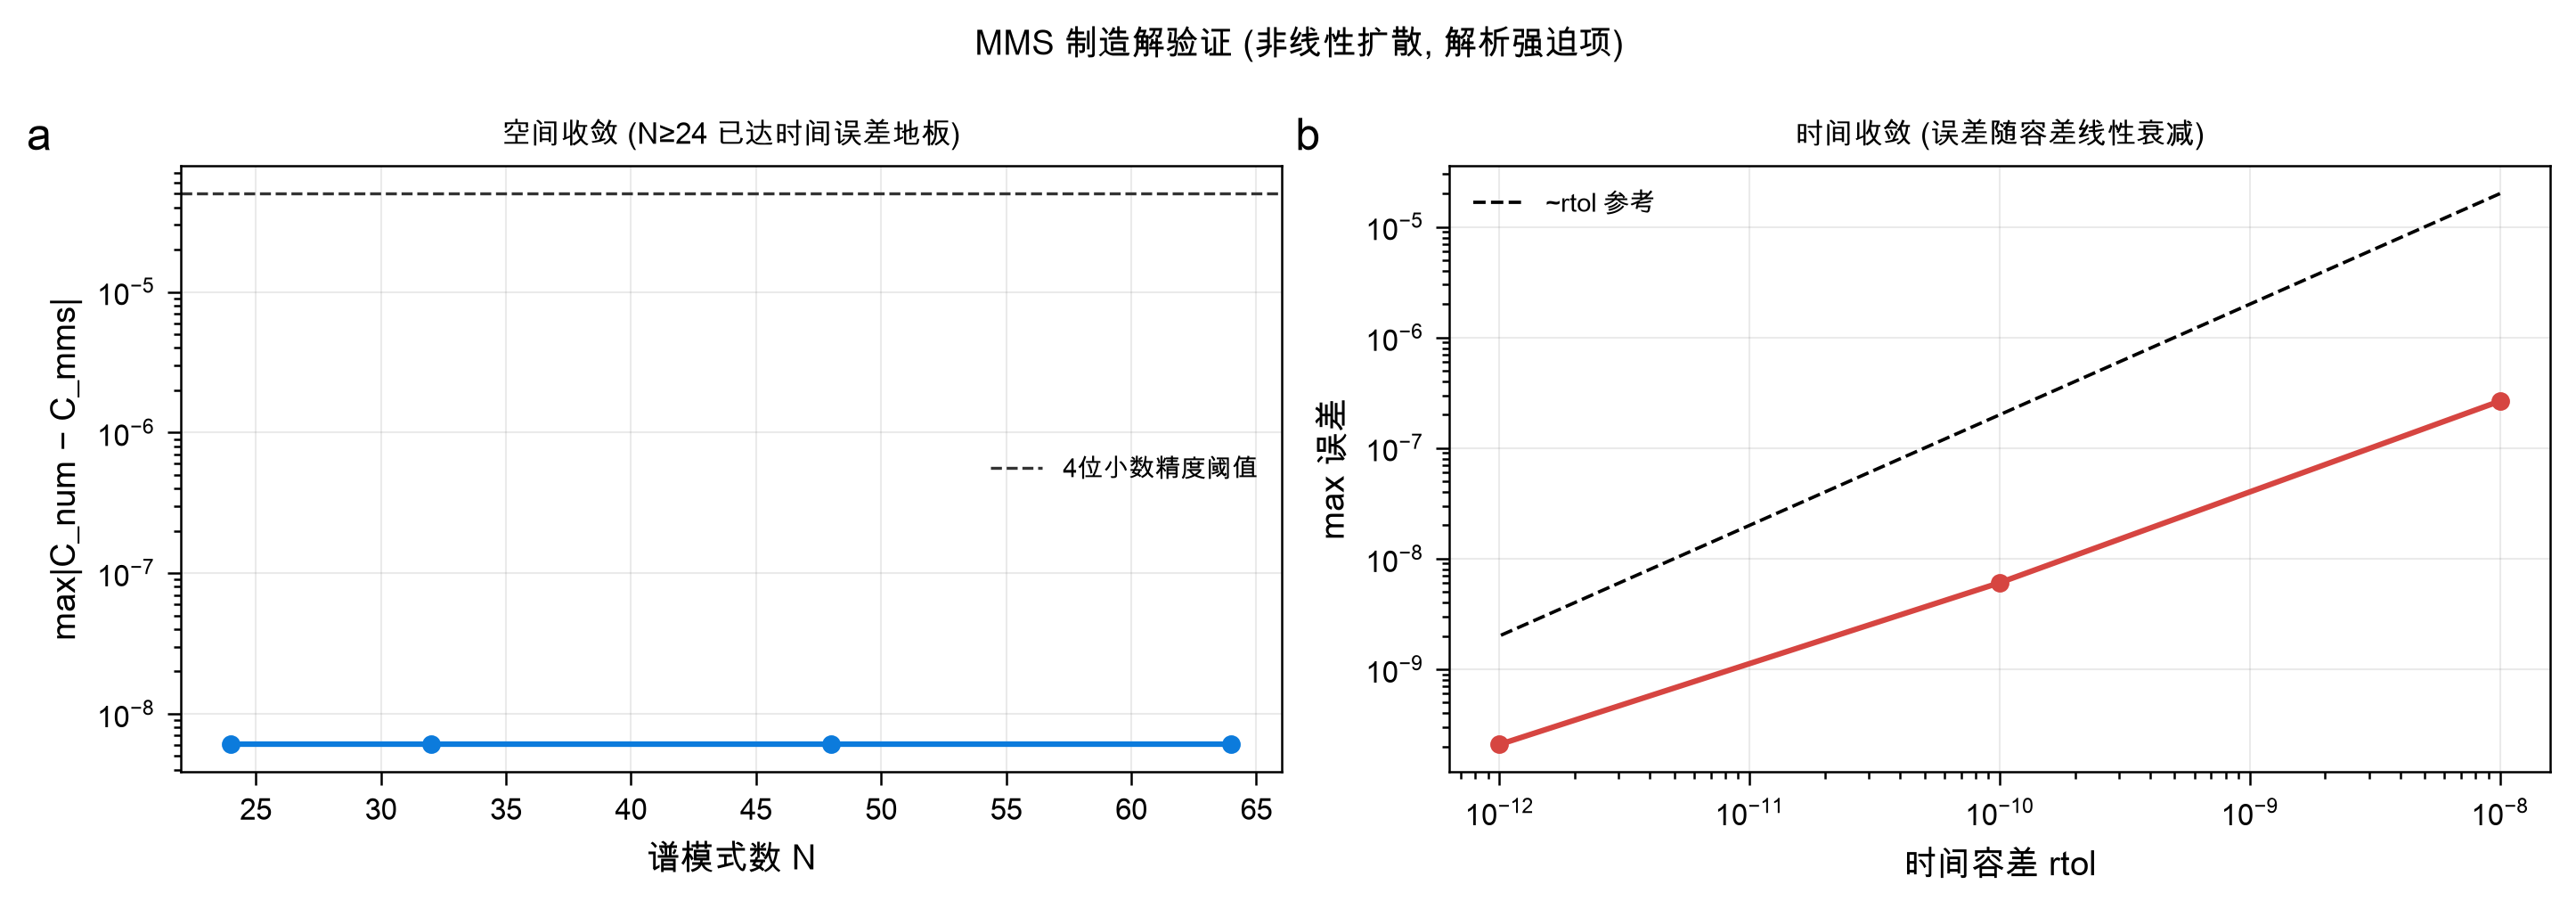
\includegraphics[width=0.95\textwidth]{fig7_mms.png}
\caption{制造解验证。（a）空间：$N\ge24$ 后谱误差低于时间误差水平；
（b）时间：误差随容差线性衰减。}
\label{fig:mms}
\end{figure}

\textbf{（2）空间与时间收敛。} 问题二给出了谱模式数 $N=48/96/128$ 的
收敛序列（表~\ref{tab:conv}），提交结果取 $N=128$；问题一末位谱系数
$5\times10^{-13}$。时间方向由 BDF 自适应控制（相对容差 $10^{-8}\sim10^{-9}$），
制造解验证确认误差随容差衰减。

\textbf{（3）独立算法交叉验证。} 全部四个问题均与独立实现的有限体积法
求解器交叉对比：问题一至三轨迹偏差 $6\times10^{-4}$ 以内、表 1--表 4
逐项 4 位小数一致；问题四与另一套坐标变换的离散结果偏差 0.02 h。两种
离散建立在不同坐标系与不同差分结构上，结果一致显著降低了由单一数值格式
或程序实现造成系统性错误的可能性（交叉验证不能替代对模型假设本身的检验，
后者见 7.2 节局限讨论）。

此外，谱配点法的边界条件在每次右端求值中由边界方程直接解出（残差
$10^{-19}$ 量级），问题四的随体网格满足几何守恒恒等式；Duhamel 解在
$\tau\to0$ 时退化为阶跃边界响应。这些内容在附录 B 中说明。

\subsection{灵敏度分析}

对五个关键参数做 OAT 单参数 $\pm10\%$ 扰动，输出指标为烘干时长
（表~\ref{tab:sens}，图~\ref{fig:tornado}）。

\begin{table}[H]
\centering
\caption{OAT 灵敏度（$\pm10\%$，QoI = 烘干时长）}
\label{tab:sens}
\begin{tabular}{ccccc}
\toprule
参数 & 名义值 & $\Delta t_{end}(-10\%)$ & $\Delta t_{end}(+10\%)$ & $|\Delta|$ 之和 \\
\midrule
$T_{bar}$（恒温段温度） & $49.969$\,°C & \textbf{+10.87 h} & \textbf{$-$8.68 h} & 19.55 h \\
$D$ 前置因子 & $2.4\times10^{-3}$ & +5.98 h & $-$4.90 h & 10.88 h \\
$\beta$（对流传质系数） & $8\times10^{-7}$ & +0.53 h & $-$0.45 h & 0.98 h \\
$h$（对流换热系数） & 25.0 & $-$0.02 h & $-$0.03 h & 0.05 h \\
\bottomrule
\end{tabular}
\end{table}

\begin{figure}[H]
\centering
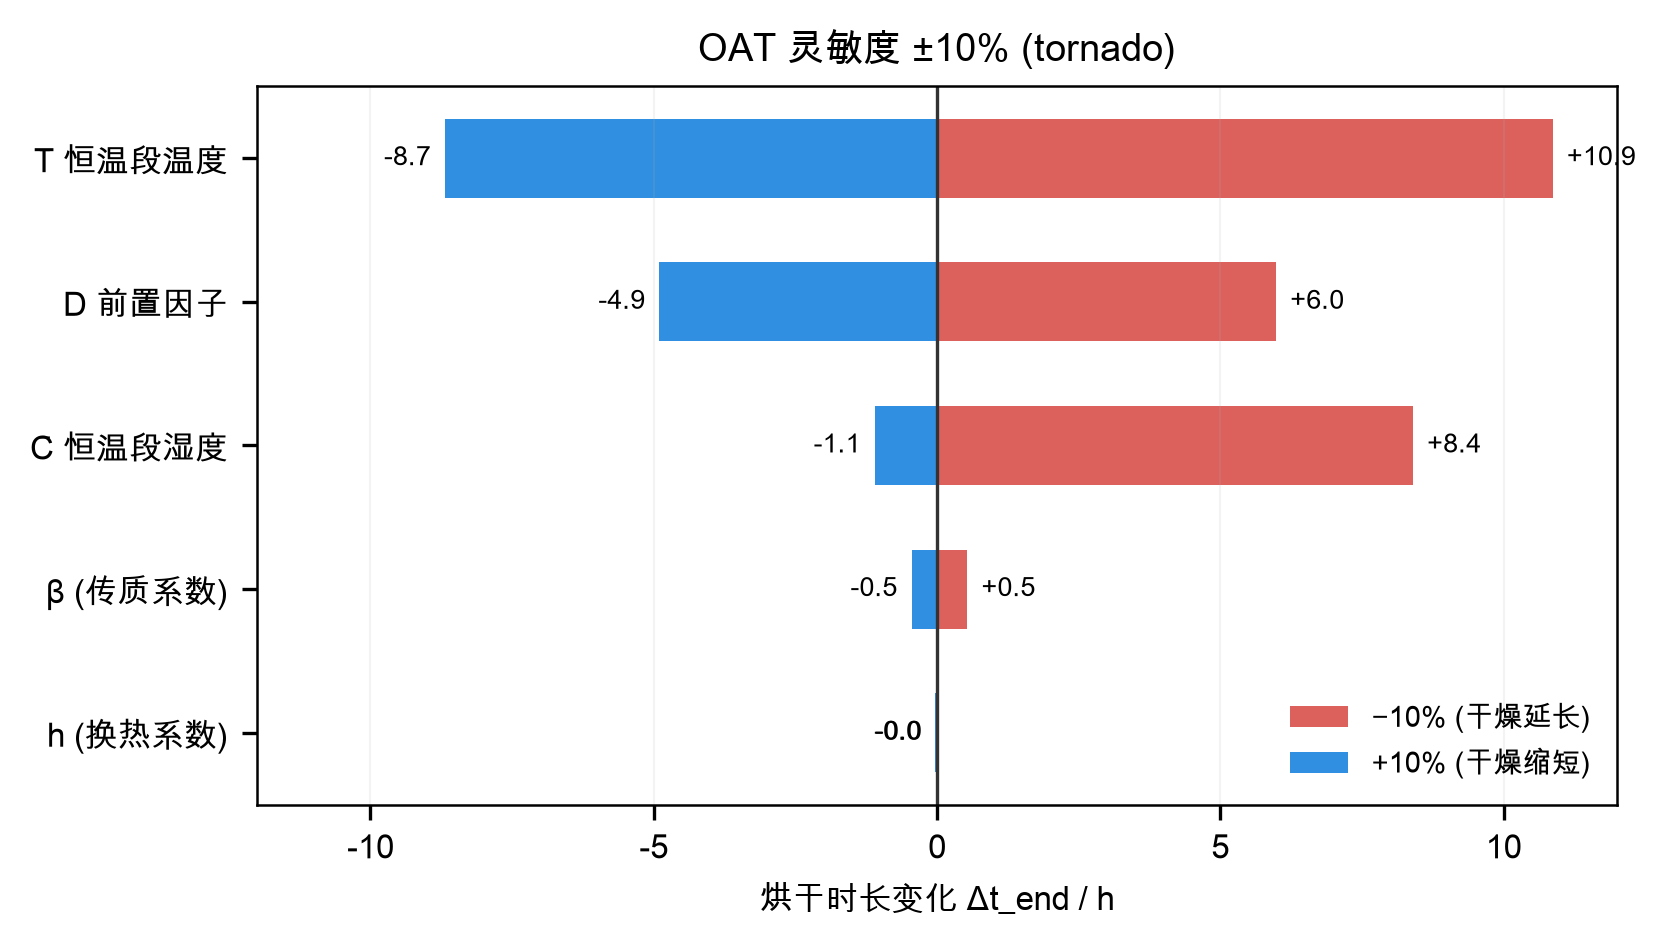
\includegraphics[width=0.72\textwidth]{fig10_tornado.png}
\caption{灵敏度 tornado 图。恒温段温度为主导控制量，换热系数影响可忽略。}
\label{fig:tornado}
\end{figure}

\textbf{解释。}\textbf{（1）温度的主导作用：}$T_{bar}$ 经 Arrhenius 项 $e^{-3850/T}$ 放大，
降温侧比升温侧更敏感（指数函数凸性所致）；\textbf{（2）传热非瓶颈：}$h$ 的影响
不足 \textbf{0.1 h}：热平衡在小时尺度内即可建立，而干燥持续数天，烘干时长由
水分扩散控制。上述四个参数两套方法给出的数值接近（有限体积法：
$T_{bar}$ $+10.40/-8.30$、$D$ 前置 $+5.73/-4.68$、$\beta$ $+0.68/-0.55$、
$h$ $\pm0.02$，单位 h），排序 $T_{bar}\gg D_{pre}>\beta>h$ 在两种方法中
一致。

\subsubsection{未收敛敏感项：恒温段湿度 $C_{bar}$}

$C_{bar}$ 的 $\pm10\%$ 扰动对空间分辨率敏感，随分辨率加密呈现单调
收敛趋势：

\begin{table}[H]
\centering
\caption{$C_{bar}-10\%$ 工况的烘干时长变化（分辨率收敛序列）}
\label{tab:cbar}
\begin{tabular}{lcc}
\toprule
方法 & 分辨率 & $\Delta t_{end}$ \\
\midrule
谱配点 & $N=96$ & $+8.40$ h \\
谱配点 & $N=128$ & $+3.17$ h \\
有限体积法 & 400 节点 & $+1.05$ h \\
\bottomrule
\end{tabular}
\end{table}

方向在全部分辨率下一致（$C_{bar}$ 降低延长干燥），幅度随分辨率加密由
8.4 h 收敛至 1--3 h 量级，但两种独立方法尚未完全一致。该工况的干燥锋面
更陡、对空间分辨率更敏感。本文将 $C_{bar}$ 单独列为未收敛敏感项，
不纳入主灵敏度排序；其定性方向（降湿延长干燥）成立，定量幅度以
1--3 h 量级估计。

% ============ §7 模型评价与推广 ============
\section{模型评价与推广}

\subsection{模型优点}

\begin{enumerate}
\item 问题一的温度场采用解析方法求解：该解在 $\tau\to0$ 时退化为阶跃
边界响应、在 $t=0$ 时恢复初值，两个极限情形均与已知解一致，并作为数值
求解器的独立基准；
\item 谱配点离散对光滑剖面指数收敛，配合末位谱系数误差指示，空间分辨率
不足时（问题二的干燥锋面）能够被直接发现并加密；
\item 问题四的随体坐标推导建立在干基含水率的物质守恒上，收缩边界处理
经另一套坐标变换独立验证；
\item 全部结果经过解析/制造解、收敛序列与独立算法三类交叉验证。
\end{enumerate}

\subsection{模型局限}

\begin{enumerate}
\item 谱方法对干燥锋面需要 $N\ge96$ 个模式（$N=48$ 时 $t_{end}$ 偏差约
14 h），二维推广时计算量增长较快；
\item 表面边界方程的求解依赖上一时刻表面值的延续，若环境条件出现阶跃式
突变需要重新论证解的连续性；
\item 问题四假设径向仿射收缩，题目仅提供径向数据，轴向与各向异性收缩
未建模；
\item 环境外推基于 0--4 h 数据，若恒温段存在更晚的工况变化，烘干时长的
偏移量以灵敏度分析（$T_{bar}$ $\pm10\%$ 对应 $-8.7\sim+10.9$ h）估计；
\item 题目参数体系未提供汽化潜热与局部相变速率，本文采用显热传导模型以
保持参数闭合，蒸发吸热对表面温度的修正未计入。
\end{enumerate}

\subsection{模型推广}

谱配点离散与随体坐标边界处理可直接推广至：片状/球状药材干燥（更换几何
因子）、果蔬脱水与粮食仓储干燥（同型有效扩散模型）、干燥工艺参数优化
（以恒温段温度为主导控制量的结论指导节能策略）。时间尺度比 $\Gamma$
的时空分布可用于干燥过程的阶段识别与工艺控制设计。


\begin{thebibliography}{99}
\bibitem{gasparin} Gasparin S, Dutykh D, Mendes N. A spectral method for solving heat and moisture transfer through consolidated porous media[J]. arXiv:1902.07775, 2019.
\bibitem{luikov} Luikov A V. Systems of differential equations of heat and mass transfer in capillary-porous bodies (review)[J]. International Journal of Heat and Mass Transfer, 1975, 18(1): 1-14.
\bibitem{trefethen} Trefethen L N. Spectral Methods in MATLAB[M]. Philadelphia: SIAM, 2000.
\bibitem{berrut} Berrut J P, Trefethen L N. Barycentric Lagrange interpolation[J]. SIAM Review, 2004, 46(3): 501-517.
\bibitem{carslaw} Carslaw H S, Jaeger J C. Conduction of Heat in Solids[M]. 2nd ed. Oxford: Clarendon Press, 1959.
\bibitem{roache} Roache P J. Code verification by the method of manufactured solutions[J]. Journal of Fluids Engineering, 2002, 124(1): 4-10.
\bibitem{erzhi} 作者待补. 二至丸热风干燥过程温度均匀性模拟与实验[J]. 中草药, 2020, 51(5): 1226-.
\bibitem{moslae} 作者待补. Effect of Drying Kinetics, Volatile Components, Flavor Changes and Final Quality Attributes of Moslae herba during the Hot Air Thin-Layer Drying Process[J]. Molecules, 2023, 28(9): 3898.
\bibitem{food} Bia\l{}obrzewski I, Zieli\'nska M, Mujumdar A S, et al. Heat and mass transfer during drying of a bed of shrinking particles---simulation for carrot cubes dried in a spout-fluidized-bed drier[J]. Drying Technology, 2008.
\bibitem{jiang} 姜启源, 谢金星, 叶俊. 数学模型[M]. 5 版. 北京: 高等教育出版社, 2018.
\end{thebibliography}

\newpage
\appendix
% ============ 附录 ============
\section{程序代码说明}

全部程序以 Python 3 实现，依赖 numpy / scipy / pandas / openpyxl / sympy，运行于 Apple M4 Pro（12 核）。代码组织：

\begin{itemize}
\item \texttt{env\_model.py}：烘房环境一阶惯性辨识（最小二乘 + PCHIP 残差 + 平台期统计）；
\item \texttt{spectral\_core.py}：Chebyshev 谱配点统一内核（CGL 微分矩阵、乘性守恒形式、谱边界消元、Newton 续延、末位系数误差估计）；
\item \texttt{q1\_analytic.py}：Duhamel 温度场闭式解析解（Robin 特征值二分求根 + 指数主项 + 残差递归卷积）；
\item \texttt{ale\_core.py}：ALE 移动网格谱配点（时变度量 + GCL 检查）；
\item \texttt{q1\_v2.py}--\texttt{q4\_v2.py}：四个子问题的驱动与输出（表 1--6、result1--4.xlsx）；
\item \texttt{mms\_v2.py}：制造解验证（sympy 解析强迫项）；
\item \texttt{sensitivity\_v2.py}：多进程并行灵敏度分析。
\end{itemize}

核心求解器（谱边界消元）关键实现摘录：

\begin{verbatim}
# 表面 Robin 条件的标量根 (Newton 续延, 沿物理支跟踪)
def _surf_moisture(self, t, y, T_surf=None):
    c_env = self.C_env_fun(t)
    A = self.DN0 * (-self.D0m @ y / self.D00) + self.DNm @ y
    B = self.DN0 * (-self.D0N / self.D00) + self.DNN
    def F(s):
        Ds = self.D_fun(np.array([s]), Ts)[0]
        return Ds * (A + B * s) + self.beta * (s - c_env)
    def dF(s):
        Ds = self.D_fun(np.array([s]), Ts)[0]
        dD = self.dDdC_fun(np.array([s]), Ts)[0]
        return dD * (A + B * s) + Ds * B + self.beta
    s = self._surf_C if self._surf_C is not None else float(np.max(y))
    ...  # Newton 迭代至 1e-13, 步出物理区间时折半
\end{verbatim}

\section{结果文件}

result1.xlsx（1800 行 $\times$ 21 列 $\times$ 2 表）、result2.xlsx（10800 行 $\times$ 21 列 $\times$ 2 表）、result3.xlsx（3470 行，60 s 至 208200 s）、result4.xlsx（3069 行，60 s 至 184140 s，末列“药材表面”，$r>R(t)$ 处留空）——均按附件 3 模板格式，4 位小数。


\end{document}
